\section{GDVND}\label{subsec:gdvnd}

Trazendo o conceito de \textit{movimentos independentes} (discutido na Seção \ref{subsubsec:movimentosIndependentes}) para o DVND surge a ideia do \emph{Generalized Distributed Variable Neighborhood Descent} (\emph{GDVND}).
A ideia do GDVND é um DVND que trabalha no escopo de movimentos de melhora e não em melhores soluções.
No DVND, a cada iteração o método recebe uma nova solução de uma das vizinhanças e verifica qual a melhor para então enviar esta para ser processada pelas vizinhanças ociosas que ainda não a processaram, sempre mantendo a melhor solução já encontrada.
A diferença para o GDVND é que este recebe não somente uma solução mas a solução com um conjunto de movimentos de melhora encontrado pela vizinhança, então o método tenta combinar os movimentos da melhor solução atual com aqueles da solução recebida.
Para tanto é necessário que as soluções tenham a mesma solução base, então é necessário identificar o conjunto de movimentos independentes que proporcione o maior ganho em termos de valor da solução.
Além de melhorar a solução a utilização da composição de movimentos proporciona uma melhor utilização dos recursos usados no processamento ao aproveitar computações realizadas em nós diferentes.

O grafo dataflow do GDVND é equivalente ao do DVND expresso na Figura~\ref{fig:dvndGraph} alterando apenas a informação trafegada entre os nós e a implementação interna do nó gerenciador, conforme Algoritmo~\ref{alg:gdvndMan}, ao qual caberá combinar os movimentos de vizinhanças diferentes.
Na linha \ref{alg:gdvndMan:merge} é chamado o processo combinar movimentos que pode ser visto em mais detalhes no Algoritmo~\ref{alg:gdvndMergeFunc}.
Os movimentos são combinados para formar uma solução resultante, tomando proveito do Teorema da independência de movimentos dois a dois (Teorema~\ref{teo:independenciaMovimentos2a2}) o valor da solução resultante pode ser calculado para dois movimentos, sem a necessidade de recalcular toda a solução, o que é particularmente útil para grandes instâncias e problemas cujo cálculo da função objetivo é muito caro computacionalmente.
Pode-se utilizar o mesmo teorema para estimar o valor das soluções na composição de mais de dois movimentos dois a dois.

\begin{algorithm}[htpb]
\caption{Nó \textit{man} do GDVND}
\label{alg:gdvndMan}
\begin{algorithmic}[1]
    \Function{GDVND\_Man}{Solução: $s$, Histórico: $H$, Vizinhança: $k$}
        \Let{$s_{merged}$}{$GDVND\_merge(s, bestSolution(H))$} \label{alg:gdvndMan:merge} \Comment{Combina a solução atual com a melhor conhecida}
        \Let{$H(k)$}{$min(s, s_{merged}, bestSolution(H))$} \Comment{Atualiza o histórico da vizinhança $k$ com a melhor solução}
        \Return{SoluçãoBase($H(k)$), Movimentos($H(k)$)}
    \EndFunction
\end{algorithmic}
\end{algorithm}

Seja um grafo $G = (V, E)$ cujos vértices $V$ são movimentos e as arestas $E$ indicam se um movimento é independente de outro.
Dessa forma encontrar o melhor sub-conjunto de movimentos independentes entre si dois a dois corresponderia a encontrar o sub-grafo completo correspondente ao clique maximal em que o o somatório do valor dos vértices seja máximo.

Neste trabalho é usada uma heurística para encontrar o melhor sub-conjunto de movimentos independentes, o Algoritmo~\ref{alg:gdvndMergeFunc} ilustra a heurística utilizada para fazer o \emph{merge} dos movimentos da solução.
O método apenas pode ser executado quando as soluções base são iguais para as duas soluções de entrada.
Os movimentos são reunidos num conjunto $M'$ e então ordenados conforme a melhoria que podem aplicar à solução.
Em seguida cada movimento é testado, em busca de conflitos, contra as demais movimentos, caso haja conflito este movimento é descartado, os movimentos foram dispostos de forma que os movimentos com pior resultado sobre a solução sejam testados primeiro, desta forma aqueles com melhores valores são deixados por último para que possam ser preservados caso possuam conflitos com algum outro.

\begin{algorithm}[htpb]
\caption{Combinando movimentos de soluções diferentes}
\label{alg:gdvndMergeFunc}
\begin{algorithmic}[1]
    \Function{GDVND\_merge}{Solução: $s_1$, Solução: $s_2$}
        \If{SoluçãoBase($s_1$) = SoluçãoBase($s_2$)} \Comment{Somente soluções com a mesma solução base podem ser combinadas}
            \Let{$M'$}{sorted(Movimentos($s_1$) $\cup$ Movimentos($s_2$))} \Comment{Movimentos ordenados pelo valor da melhoria na solução}
            \For{$i \gets 0$ to $len(M')$}
                \For{$j \gets (i + 1)$ to $len(M')$}
                    \If{$m_i \nparallel m_j$}
                        \Let{$M'$}{$M' - {m_i}$}
                        \State break
                    \EndIf
                \EndFor
            \EndFor
            \Return{SoluçãoBase($s_1$), $M'$}
        \EndIf
        \Return{$min(s_1, s_2)$}
    \EndFunction
\end{algorithmic}
\end{algorithm}

O retorno da iteração de cada vizinhança do GDVND passa a corresponder não a uma solução $s'$ mas a uma tupla com a solução e os movimentos aplicados, assim temos a resposta como $(s', \{m_1^x, m_2^x, \dots, m_k^x\})$.

É importante ressaltar a diferença do \emph{Multi Improvement} para o GDVND, o primeiro é uma estratégia de exploração de vizinhanças em que a busca local avança de uma solução para outra fazendo uso de uma composição de movimentos independentes $\{m_1^x, m_2^x, \dots, m_k^x\} \subset M^x$ pertencentes a uma vizinhança, no caso do GDVND os movimentos independentes são oriundos de todas as vizinhanças utilizadas pelo algoritmo.
Ainda na analogia com o \emph{Multi Improvement}, o GDVND poderia ser visto como um \emph{multi improvement} em que a sua vizinhança é a união de todas as vizinhanças utilizadas no GDVND.

A mesma ideia pode ser aplicada para um conjunto de movimentos $M = \{ m_1, m_2, m_3, ...\}$, ditos independentes se para uma solução $s$ qualquer e para todo subconjunto não-vazio $M' = \{ m_1, m_2, m_3, ..., m_k \} \subseteq M$ temos $\widehat{m_1}(s) + \widehat{m_2}(s) + \widehat{m_3}(s) + ... + \widehat{m_k}(s) = \widehat{m_1}(m_2 \circ m_3 \circ ...\circ m_k \circ s)$. 
Utilizaremos a letra $I$ para denotar movimentos independentes, por exemplo, $I(\{m_3, m_5, m_9\})$.

\subsection{Detecção movimentos independentes} \label{subsec:gdvndDetectarMovimentosIndependentes}

Para detectar quais movimentos são independentes, uma estrutura de dados $C$ para gerenciamento de conflitos foi proposta.
No caso do problema em questão, a estrutura se trata de vetor com $N$ bits, onde cada bit $i$ indica se houve alguma alteração relativa ao cliente $i$.

Exemplo $C: |0|0|0|1|1|1|1|0|0|0|0|0|0|$

Assim, a estrutura $C$ começa com todos bits zero, considerando uma solução de referência $s$.
Cada movimento altera a estrutura $C$ além de alterar a solução corrente, indicando quais posições estão comprometidas.
Da mesma maneira, uma função $d$ de detecção de conflitos indica se um movimento é "aplicável" dada certa configuração da estrutura de conflitos.

Dessa forma, ao aplicar um movimento, se for necessário alterar um bit para 1 que já tenha valor 1 então o movimento atual é conflitante com o anterior ou algum dos anteriores.

Como podemos ver a seguir a detecção de conflitos para uma solução de tamanho $n=13$, os movimentos $Swap_{1,3} \parallel Swap_{5,9}$, $Swap_{5,9} \parallel Swap_{3,7}$ mas $Swap_{1,3} \nparallel Swap_{3,7}$.\\
$C:$ |0|\textbf{0}|0|\textbf{0}|0|0|0|0|0|0|0|0|0| - $Swap_{1,3}$ \\
$C:$ |0|1|0|1|0|\textbf{0}|0|0|0|\textbf{0}|0|0|0| - $Swap_{5,9}$ \\
$C:$ |0|1|0|\textbf{1}|0|1|0|\textbf{0}|0|1|0|0|0| - $Swap_{3,7}$ \\
$C:$ |0|1|0|\textcolor{red}{0}|0|1|0|1|0|1|0|0|0| - Conflito \\
A estrutura começa com todos os bits com valor zero, os bits em negrito indicam aqueles que serão alterados pelo movimento atual, na última linha o bit em vermelho indica a existência de um conflito ($Swap_{1,3} \nparallel Swap_{3,7}$).

\subsection{Exemplo de execução} \label{subsec:gdvndExemplo}

No DVND, várias buscas começam de uma mesma solução de referência e o melhor movimento (ou primeiro de melhora) é retornado como candidato à inclusão em um pool de movimentos, chamado Histórico.
Este pool pode ser visto como um grafo não direcionado, no qual os vértices são movimentos e arestas indicam conflitos entre movimentos.
Porém, setas especiais são utilizadas para marcar dependência entre movimentos. Se $m_B$ depende de $m_A$, então $m_B$ só pode ser aplicado se $m_A$ for aplicado antes na solução.
Escolhendo o maior (ou menor) conjunto independente neste grafo, respeitando os conflitos e dependências, resultará na melhor combinação de movimentos em um dado momento, considerando múltiplas estruturas de vizinhança simultaneamente.

A Figura~\ref{fig:exemplo-dvnd} apresenta um exemplo do grafo de Histórico para uma execução do GDVND com três processos de busca.

\begin{figure}[htpb]
    \centering
    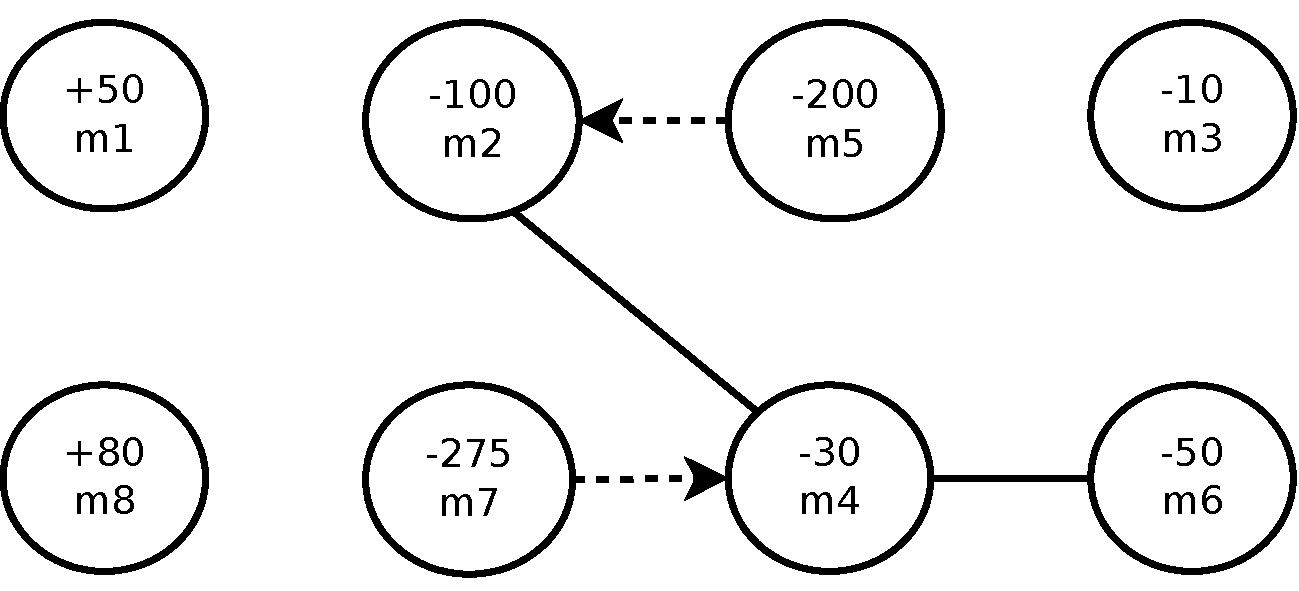
\includegraphics[width=0.65\linewidth]{figuras/gdvnd/dvnd_exemp.pdf}
    \caption{Exemplo de um grafo de Histórico.
    A combinação ótima de custos consiste nos movimentos $m_2$, $m_3$, $m_5$ e $m_6$.
    \label{fig:exemplo-dvnd}}
\end{figure}

Para entender melhor a ideia do algoritmo, a tabela abaixo simula a execução do algoritmo para três processos.

\begin{table}[htpb]
\centering
\caption{Execução do GDVND}
\begin{tabular}{|c|cccc|c|}
\hline
    \# & $f$ & solução & direção & processo & conflito\\\hline
    1  & 1000 & $s_1$ & $\rightarrow$ & P1 &\\
    2  & 1000 & $s_1$ & $\rightarrow$ & P2 &\\
    3  & 1000 & $s_1$ & $\rightarrow$ & P3 &\\\hline
    4  & 970 & $m_4 \circ s_1$ & $\leftarrow$ & P3 &\\
    5  & 970 & $m_4 \circ s_1$ & $\rightarrow$ & P3 &\\\hline
    6  & 900 & $m_2 \circ s_1$ & $\leftarrow$ & P1 & \\
    7*  & 900 & $m_2 \circ s_1$ & $\rightarrow$ & P1 & $m_2 \nparallel m_4$\\\hline
    8  & 1050 & $m_1 \circ s_1$ & $\leftarrow$ & P2 &\\
    9*  & 900 & $m_2 \circ s_1$ & $\rightarrow$ & P2 &\\\hline
    10 & 890 & $m_3 \circ m_2 \circ s_1$ & $\leftarrow$ & P1 & \\
    11 & 890 & $m_3 \circ m_2 \circ s_1$ & $\rightarrow$ & P1 & $m_2 \parallel m_3$\\\hline
    12 & 700 & $m_5 \circ m_2 \circ s_1$ & $\leftarrow$ & P2 &\\
    13 & 690 & $m_5 \circ m_3 \circ m_2 \circ s_1$ & $\rightarrow$ & P2 & $m_3 \parallel m_5$ e $m_2 \parallel m_5$\\\hline
    14 & 695 & $m_7 \circ m_4 \circ s_1$ & $\leftarrow$ & P3 &\\
    15 & 685 & $m_7 \circ m_4 \circ m_3 \circ s_1$ & $\rightarrow$ & P3 & $m_2 \nparallel m_7$ e $m_5 \nparallel m_4$\\\hline
    16 & 840 & $m_6 \circ m_3 \circ m_2 \circ s_1$ & $\leftarrow$ & P1 &\\
    17 & 640 & $m_6 \circ m_3 \circ m_5 \circ m_2 \circ s_1$ & $\rightarrow$ & P1 & $m_6 \parallel m_2, m_3, m_5$\\\hline
    18 & 765 & $m_8 \circ m_7 \circ m_4 \circ m_3 \circ s_1$ & $\leftarrow$ & P3 &\\
    19 & 640 & $m_6 \circ m_3 \circ m_5 \circ m_2 \circ s_1$ & $\rightarrow$ & P3 & $m_8 \nparallel m_6$\\\hline
\end{tabular}
\end{table}

O Histórico começa distribuindo a solução $s_1$ para cada busca, e eventualmente coleta um novo movimento e distribui uma nova solução.
Todos os cálculos são feitos sobre uma mesma solução de referência $s_1$, que só é modificada no passo 20 do algoritmo.
Nas iterações 7 e 9, note que existem conflitos a serem resolvidos (vide grafo na Figura~\ref{fig:exemplo-dvnd}).
Após a iteração 19, o Histórico percebe que os três processos tem movimentos em comum: $m_3$, $m_5$ e $m_2$. Então uma nova solução $s_2$ é armazenada no Histórico como solução de referência, sendo ela $s_2 = m_3 \circ m_5 \circ m_2 \circ s_1$ (de custo 690).
Assim, os processos P1 e P3 continuam naturalmente processando a solução $m_6 \circ s_2$ (antiga $m_6 \circ m_3 \circ m_5 \circ m_2 \circ s_1$), e P2 continua com $s_2$ (antiga $m_5 \circ m_3 \circ m_2 \circ s_1$).
Note também que, ao adotar estes três movimentos, todos movimentos com conflitos (ou dependência de algum movimento em conflito) tem de ser eliminados. Então, $m_4$ e $m_7$ são descartados.
Vale observar que $m_1$ e $m_8$ nunca foram armazenados, pois eram de piora.
O grafo final então consiste somente dos movimentos $m_6$, $m_3$, $m_5$ e $m_2$.

%OBSERVAÇÃO IMPORTANTE: eu acho que este processo pode ser mais estável se a unificação ocorrer após UMA iteração que o conjunto de movimentos comuns se mantenha estável, mas teremos que experimentar para saber =D

\begin{table}[htpb]
\centering
\caption{Consolidação de uma nova solução no GDVND}
\begin{tabular}{|c|ccc|}
\hline
\# & $f$ & solução & local\\\hline
20 & 690 & $s_2 = m_3 \circ m_5 \circ m_2 \circ s_1$ &  Histórico\\
   & 640 & $m_6 \circ s_2$ & P1\\
   & 690 & $s_2$           & P2\\
   & 640 & $m_6 \circ s_2$ & P3\\\hline
\end{tabular}
\end{table}

\subsection{Controle de execução entre CPU e GPU}

Para entender como o método tira proveito da arquitetura híbrida CPU-GPU segue o presente exemplo:
A CPU é utilizada para decidir qual solução cada processo de busca local irá utilizar, minimizando as transferências de memória CPU-GPU. % e, assim, maximizando o aproveitamento na estrutura de dados ADS (informações auxiliares usada para acelerar o cálculo do valor da solução) das na memória da GPU.

EXEMPLO:\\
 Processo A $\rightarrow$ CPU\\
 Processo B $\rightarrow$ Kernel GPU Swap\\
 Processo C $\rightarrow$ Kernel GPU 2-Opt\\
 Processo D $\rightarrow$ Kernel GPU Or-1\\
 Processo E $\rightarrow$ Kernel GPU Or-2\\
 Processo F $\rightarrow$ Kernel GPU Or-3

Solução $s_1$ = [1,2,3,4,5,6,7,8,9,10], ($f(s_1) = 1000$).

A solução $s_1$ entra na GPU para todas as buscas B-F, cada uma em um fluxo (\emph{thread}) distinto.
Supomos que o processo B (Swap) termina antes com ganho -100 (melhora, $\widehat{m_1} = -100$) na troca $m_1 = Swap_{2,5}$.
A CPU então cria $s_2 = m_1 \circ s_1$.
Como $s_2$ é a melhor solução atual, ela é copiada para a GPU, e o processo B roda em cima de $s_2$ = [1,5,3,4,2,6,7,8,9,10], com $f(s_2) = 900$.

Neste momento, o processo D termina com $m_2 = Or-1_{7,9}$, movendo cliente 7 para depois do 9, com ganho -50, $\widehat{m_2} = -50$.
A CPU então analisa $m_1$ e $m_2$, como não há conflitos uma solução $s_3 = m_2 \circ m_1 s_1$ é criada para o processo D executar. $s_3$=[1,5,3,4,2,6,8,9,7,10], com $f(s_3) = 850$

O processo C termina com o movimento $m_3=2Opt_{1,3}$ (inverte de 1 a 3) com ganho -120 ($\widehat{m_3} = -120$.
A CPU percebe que $m_3 \nparallel m_1$, mas $m_3 \parallel m_2$.
Então a solução $s_4= m_4 \circ m_2 \circ s_1$ é gerada e passada à GPU para o processo C, com $f(s_4) = 830$

O processo E termina sem ganho com o movimento $m_4 = Or-2_{1,4}$ (move clientes 1,2 para depois do 4).
A CPU percebe que $m_4 \nparallel m_1$ e $m_4 \nparallel m_3$ mas $m_4 \parallel m_2$.
Porém, a melhor configuração atual é $s_4$ ($f(s_4)=830$), então a busca parte dela (e ela já está na memória da GPU).

Finalmente, o processo B (Swap) termina novamente com melhora -60 e troca $m_5=Swap_{3,8}$.
Esta troca roda em cima de $s_2$, então não existem outros movimentos para haver conflito.
A solução $s_5 = m_5 \circ s_2$ com $f(s_5) = 840$ é criada, porém, a solução $s_4$ ($f(s_4) = 830$) é melhor.
A CPU então relança o processo B com a solução $s_4$.

\subsubsection{Passo iterativo}

Utilizando o termo convencionado na seção~\ref{subsec:passoIterativo}, cada passo iterativo do GDVND retorna a melhor solução encontrada para todas as vizinhanças combinado com a melhor solução já encontrada.
Dessa forma, sendo $N$ a união de todas as vizinhanças, contudo a resposta do GDVND pode conter mais de um movimento combinados simultaneamente, assim convencionaremos chamar de $\mathcal{N} = \{ m_1 \circ m_2 \circ \dots \circ m_z \circ s \mid \forall m_i \in \mathcal{M} \land \forall i, j \quad m_i \parallel m_j \}$, podemos ver, pela definição de $\mathcal{N}$, que $N \subset \mathcal{N}$ pois qualquer elemento de $N$ pode ser escrito da forma $m_1 \circ s$ que também pertence a $\mathcal{N}$.
Assim o passo iterativo do GDVND pode ser dado pela Equação~\ref{eq:gdvndPassoIterativo}.

\begin{equation} \label{eq:gdvndPassoIterativo}
\rho^{GDVND}(s) = s' \in \mathcal{N} \  \textrm{sendo} \  f(s') < f(s''), \forall s'' \in \mathcal{N}(s) \  \textrm{com} \  s'' \ne s
\end{equation}

Fazendo uso da notação de movimentos podemos escrever \ref{eq:dvndPassoIterativo} como a Equação~\ref{eq:dvndPassoIterativoMovimento}.

\begin{equation} \label{eq:gdvndPassoIterativoMovimento}
\rho^{GDVND}(s) = m_1 \circ m_2 \circ \dots \circ m_z \circ s \  \textrm{sendo} \  m \in \mathcal{M} \land \forall i,j \quad m_i \parallel m_j \  \textrm{com} \  i \ne j
\end{equation}

Pelo passo iterativo do RVND $\rho^{RVND}$ (\ref{eq:rvndPassoIterativoMovimento}), do DVND $\rho^{DVND}$ (\ref{eq:dvndPassoIterativoMovimento}) e do GDVND $\rho^{GDVND}$ (\ref{eq:gdvndPassoIterativoMovimento}) podemos concluir que $\rho^{GDVND}(s) \le \rho^{DVND}(s) \le \rho^{RVND}(s)$, contudo novamente isso não é suficiente para afirmar que o GDVND encontre necessariamente melhores resultados pois o pode acabar convergindo muito cedo para um mínimo local.

À primeira vista pode parecer que pela vizinhança do passo iterativo do GDVND conter as vizinhanças do RVND e DVND contudo podemos ver que toda solução encontrada pelo GDVND pode ser gerada por um conjunto de operações do DVND ou RVND.

Para que uma solução produzida pelo GDVND não possa ser produzida pelo RVND ou DVND deve haver um movimento nessa solução que não seja possível encontrar com RVND ou DVND, suponhamos então que o GDVND produziu uma solução $m_1 \circ m_2 \circ \dots \circ m_z \circ s \in \mathcal{N}$ com $m_i \in \{ m_1, m_2, \dots, m_z \}$ tal que $m_i \notin \mathcal{M}$.
\begin{proof}
\begin{align*}
\rho^{GDVND}(s) =& m_1 \circ m_2 \circ \dots \circ m_i \circ \dots \circ m_z \circ s & \textrm{Por comutatividade} \\
\rho^{GDVND}(s) =& m_i \circ m_1 \circ m_2 \circ \dots \circ m_z \circ s & \textrm{Fazendo } s' = m_1 \circ m_2 \circ \dots \circ m_z \circ s \\
\rho^{GDVND}(s) =& m_i \circ s' & \textrm{Logo uma contradição } \bot \\
\end{align*}
\end{proof}
Quando se escreve $\rho^{GDVND}(s) = m_i \circ s'$ chega-se a uma contradição pois, pela definição do passo iterativo do GDVND, temos que o movimento $m_i$ deveria pertencer ao conjunto $\mathcal{M}$ contudo supôs-se por hipótese que $m_i \notin \mathcal{M}$.
